\documentclass{article}
\usepackage{graphicx} % Required for inserting images
\usepackage{amsmath}
\usepackage{float}
\usepackage{comment}
\usepackage{amssymb}
\usepackage{mathtools}
\usepackage{makecell}

\DeclareMathOperator*{\argmin}{arg\,min}



\title{ELEN090-2 Information And Coding Theory \\
Project 1: Information measures}
\author{Sébastien Laurent (s201561) - Duy Vu Dinh (s2401627)}
\date{}

\begin{document}

\maketitle

\section{Implementation}

\subsection{Question 1}

\subsubsection*{Mathematical formula}

The entropy $H(\mathcal{X})$ of a random variable $\mathcal{X} = \{X_1, X_2, \ldots, X_n\}$ from its probability distribution $P_\mathcal{X} = (p_1, p_2, \ldots, p_n)$ is defined as:

\begin{equation}
\label{eq:entropy}
H(\mathcal{X}) \triangleq \ - \sum_{i=1}^{n} p_i \log_2 p_i
\end{equation}

where:
\begin{itemize}
    \item $p_i \in [0, 1]$ represents the probability of each possible event $X_i$, the $i$-th possible element of $X$.
    \item The logarithm $log_2 p_i$ is taken in base 2, ensuring that entropy is measured in bits (or Shannon bits).
    \item Since $p_i \in [0, 1]$, $log_2 p_i \leq 0$. Therefore, the negative sign ensures that the entropy is non-negative. In other words, $H(\mathcal{X}) \geq 0$.
    % \item If any $i$-th event $p_i = 0$, then $p_i \log_2 p_i$ is defined as 0, since $\lim_{p \to 0} p \log_2 p = 0$.
    \item If some events have zero probability, i.e., \( p_i = 0 \), we can calculate the entropy by excluding them from the sum, which means assuming \( p_i \log_2 p_i \equiv 0 \), since \( \lim_{p \to 0} p \log_2 p = 0 \).

\end{itemize}

\subsubsection*{Explanation of implementation}

The function \texttt{entropy(Px)} operates in the following manner:

\begin{itemize}
    \item \texttt{where=(Px > 0)}: Ensures zero-probability events are ignored, implementing the mathematical limit convention.
    \item \texttt{-np.sum(Px * np.log2(Px))}: Computes the entropy. First, each probability $p_i$ is multiplied by its log value $\log_2 p_i$ for all $i$, then we sum over all terms and negate the sum to ensure we get the non-negative entropy value.
\end{itemize}

\subsubsection*{Intuitive interpretation}

Intuitively, the entropy measures the average information provided by the random variable. In other words, it measures the amount of uncertainty in a random variable.
\begin{itemize}
    \item High entropy: The distribution is more random and the variable is highly unpredictable (e.g. uniform distribution). If $p_1 = p_2 = \ldots = p_n$, i.e. $p_i = \frac{1}{n}$, then the entropy $H(\mathcal{X})$ is maximum. This means that if all outcomes are equally likely, entropy is maximized.
    \item Low entropy: The outcome is more predictable. If $p_i = 1$ (one event has the probability of 1), then the entropy $H(\mathcal{X}) = 0$, i.e. there is no uncertainty.
\end{itemize}

\subsection{Question 2}

\subsubsection*{Mathematical formula}
The joint entropy $H(\mathcal{X},\mathcal{Y})$ of two discrete random variables $\mathcal{X} = \{X_1, X_2, \ldots, X_n\}$ and $\mathcal{Y} = \{Y_1, Y_2, \ldots, Y_m\}$ with joint probability distribution $P_{\mathcal{X},\mathcal{Y}}$ is defined as:

\begin{equation}
H(\mathcal{X},\mathcal{Y}) \triangleq - \sum_{i=1}^{n} \sum_{j=1}^{m} P(X_i, Y_j) \log_2 P(X_i, Y_j)
\end{equation}


where:
\begin{itemize}
    \item $P(X_i, Y_j)$ is the probability of the joint event $\mathcal{X} = X_i$, $\mathcal{Y} = Y_j$. $$P(X_i, Y_j) = P(X_i) P(Y_j|X_i) = P(Y_j) P(X_i|Y_j) = P(X_i \cap Y_j)$$
\end{itemize}

\subsubsection*{Explanation of implementation}

\begin{itemize}
    \item \texttt{where=(Pxy > 0)}: Ensures zero-probability events are ignored, implementing the mathematical limit convention.
    \item \texttt{-np.sum(Pxy * np.log2(Pxy))} computes the joint entropy. First, each probability $p_{ij}$ is multiplied by its log value $\log_2 p_{ij}$, then we sum over all terms and negate the sum to ensure we get the non-negative joint entropy value.
\end{itemize}

\subsubsection*{Comparison between entropy and joint entropy}
\begin{itemize}
    \item The joint entropy simply amounts to setting $\mathcal{Z} = (\mathcal{X}, \mathcal{Y})$ and applying the definition of entropy (eq. \ref{eq:entropy}) to this new random variable, whose possible values are the combinations of the values of $\mathcal{X}$ and $\mathcal{Y}$.
    \item Entropy $H(\mathcal{X})$ measures the uncertainty of a single random variable, while joint entropy $H(\mathcal{X},\mathcal{Y})$ measures the combined uncertainty of two random variables.
\end{itemize}

\begin{equation}
H(\mathcal{X},\mathcal{Y}) = H(\mathcal{X}) + H(\mathcal{Y} | \mathcal{X}) = H(\mathcal{Y}) + H(\mathcal{X} | \mathcal{Y})
\end{equation}

\begin{itemize}
    % \item $H(\mathcal{X},\mathcal{Y}) = H(\mathcal{X}) + H(\mathcal{Y})$ iff $\mathcal{X} \perp \mathcal{Y}$.
    \item $H(\mathcal{X},\mathcal{Y}) \leq H(\mathcal{X}) + H(\mathcal{Y})$ with equality iff $\mathcal{X} \perp \mathcal{Y}$.
    \item $H(\mathcal{X},\mathcal{Y}) \geq \max \{H(\mathcal{X}), H(\mathcal{Y})\}$
\end{itemize}

\subsection*{Question 3}

\subsubsection*{Mathematical formula}

The conditional entropy $H(\mathcal{X} | \mathcal{Y})$ of a discrete random variable $\mathcal{X} = \{X_1, X_2, \ldots, X_n\}$ given another discrete random variable $\mathcal{Y} = \{Y_1, Y_2, \ldots, Y_m\}$, with joint probability distribution $P_{\mathcal{X},\mathcal{Y}}$, is defined as:

\begin{equation}
H(\mathcal{X} | \mathcal{Y}) \triangleq - \sum_{i=1}^{n} \sum_{j=1}^{m} P(X_i, Y_j) \log_2 P(X_i | Y_j)
\end{equation}

where:
\begin{itemize}
    \item $P(X_i, Y_j)$ is the joint probability of $X_i$ and $Y_j$.
    \item $P(X_i | Y_j) = \frac{P(X_i, Y_j)}{P(Y_j)}$ is the conditional probability of $X_i$ given $Y_J$.
    \item $P(Y_j)$ is the marginal probability of $\mathcal{Y}$.
    \item The logarithm is taken in base 2 to measure entropy in bits.
\end{itemize}

\subsubsection*{Explanation of implementation}

The implementation follows Eq. (\ref{eq:conditional_entropy_relation}):
\begin{itemize}
    \item \texttt{joint\_entropy(Pxy)}: Computes the joint entropy $H(\mathcal{X}, \mathcal{Y})$, introduced in question 2.
    \item \texttt{np.sum(Pxy, axis=0)}: Computes the marginal probability distribution $P(Y_j)$ by summing over all $X_i$.
    \item \texttt{entropy(np.sum(Pxy, axis=0))}: Computes the entropy $H(\mathcal{Y})$, introduced in question 1.
\end{itemize}

% \begin{itemize}
%     \item \texttt{np.sum(Pxy, axis=0)} computes the marginal probability distribution of $Y_i$.
%     \item \texttt{Pxy / np.sum(Pxy, axis=0)} computes the conditional probability $P(\mathcal{X} | \mathcal{Y})$.
% \end{itemize}

\subsubsection*{Equivalent way of computing that quantity}

An equivalent formula for conditional entropy is:

\begin{equation}
\label{eq:conditional_entropy_relation}
H(\mathcal{X} | \mathcal{Y}) = H(\mathcal{X}, \mathcal{Y}) - H(\mathcal{Y})
\end{equation}

where:
\begin{itemize}
    \item $H(\mathcal{X}, \mathcal{Y})$ is the joint entropy of $\mathcal{X}$ and $\mathcal{Y}$.
    \item $H(\mathcal{Y})$ is the entropy of $\mathcal{Y}$.
\end{itemize}

\subsection*{Question 4}

\subsubsection*{Mathematical formula}

The mutual information $I(\mathcal{X};\mathcal{Y})$ between two discrete random variables $\mathcal{X}$ and $\mathcal{Y}$ with joint probability distribution $P_{\mathcal{X},\mathcal{Y}}$ is defined as:

\begin{equation}
\mathcal{I(\mathcal{X};\mathcal{Y})} = \sum_{i=1}^{n} \sum_{j=1}^{m} P(X_i, Y_j) \log_2 \frac{P(X_i, Y_j)}{P(X_i) P(Y_j)}
\end{equation}

where:
\begin{itemize}
    \item $P(X_i, Y_j)$ is the joint probability distribution of $\mathcal{X}$ and $\mathcal{Y}$.
    \item $P(X_i) = \sum_{j} P(X_i, Y_j)$ is the marginal probability of $\mathcal{X}$.
    \item $P(Y_j) = \sum_{i} P(X_i, Y_j)$ is the marginal probability of $\mathcal{Y}$.
\end{itemize}

\subsection*{Explanation of implementation}

The implementation follows Eq. (\ref{eq:mutual_info_related_to_entropy}):
\begin{itemize}
    \item \texttt{np.sum(Pxy, axis=1)}: Computes the marginal probability distribution $P(\mathcal{X})$ by summing over $Y$.
    \item \texttt{entropy(np.sum(Pxy, axis=1))}: Computes the entropy $H(\mathcal{X})$, introduced in question 1.
    \item \texttt{conditional\_entropy(Pxy)}: Computes $H(\mathcal{X} | \mathcal{Y})$, introduced in question 3.
\end{itemize}

% \begin{itemize}
%     \item \texttt{np.sum(Pxy, axis=1)} computes the marginal probability of $X$.
%     \item \texttt{np.sum(Pxy, axis=0)} computes the marginal probability of $Y$.
%     \item \texttt{Pxy / (np.sum(Pxy, axis=1)[:, None] * np.sum(Pxy, axis=0))} calculates the ratio $\frac{P(\mathcal{X}, \mathcal{Y})}{P(\mathcal{X}) P(\mathcal{Y})}$.
% \end{itemize}

\subsection*{Interpretation of mutual information}

Mutual information $I(\mathcal{X};\mathcal{Y})$ measures the reduction in uncertainty about $\mathcal{X}$ given that we know $\mathcal{Y}$. It quantifies the dependency between $\mathcal{X}$ and $\mathcal{Y}$. In other words, Higher values of $I(\mathcal{X};\mathcal{Y})$ indicate stronger relationships (or higher correlation) between $X$ and $Y$:
\begin{equation}
    I(\mathcal{X};\mathcal{Y}) = H(\mathcal{X}) - H(\mathcal{X}|\mathcal{Y}) = H(\mathcal{Y}) - H(\mathcal{Y}|\mathcal{X})
\label{eq:mutual_info_related_to_entropy}
\end{equation}
\begin{itemize}
    \item $I(\mathcal{X};\mathcal{Y}) \geq 0$ with equality iff $\mathcal{X} \perp \mathcal{Y}$.
    \item $I(\mathcal{X};\mathcal{Y}) \leq \min \{H(\mathcal{X}), H(\mathcal{Y})\}$ with equality of $I(\mathcal{X};\mathcal{Y}) = H(\mathcal{X})$ iff $\mathcal{Y} = g(\mathcal{X})$.
\end{itemize}

\subsection*{Question 5}

\subsubsection*{Mathematical formula}

The conditional joint entropy $H(\mathcal{X}, \mathcal{Y} | \mathcal{Z})$ quantifies the remaining uncertainty of $(\mathcal{X},\mathcal{Y})$ given that $\mathcal{Z}$ is known. It is defined as:

\begin{align}
H(\mathcal{X}, \mathcal{Y} | \mathcal{Z}) &= - \sum_{i=1}^{n} \sum_{j=1}^{m} \sum_{k=1}^{l} P(X_i, Y_j, Z_k) \log_2 P(X_i, Y_j | Z_k) \\
&= - \sum_{i=1}^{n} \sum_{j=1}^{m} \sum_{k=1}^{l} P(X_i, Y_j, Z_k) \log_2 \frac{P(X_i, Y_j, Z_k)}{P(Z_k)} \\
&= H(\mathcal{X}, \mathcal{Y}, \mathcal{Z}) - H(\mathcal{Z}) \\
&= H(\mathcal{X} | \mathcal{Z}) + H(\mathcal{Y} | \mathcal{X}, \mathcal{Z}) \\
&= H(\mathcal{Y} | \mathcal{Z}) + H(\mathcal{X} | \mathcal{Y}, \mathcal{Z})
\end{align}

where:
\begin{itemize}
    \item $P(X_i, Y_j, Z_k)$ is the joint probability of $(\mathcal{X},\mathcal{Y},\mathcal{Z})$.
    \item $P(X_i, Y_j | Z_k) = \frac{P(X_i, Y_j, Z_k)}{P(Z_k)}$ is the conditional probability.
\end{itemize}

The conditional mutual information $\mathcal{I(\mathcal{X};\mathcal{Y} | \mathcal{Z})}$ measures the information shared between $\mathcal{X}$ and $\mathcal{Y}$ when $\mathcal{Z}$ is known:



\begin{align}
I(\mathcal{X};\mathcal{Y} | \mathcal{Z}) &\triangleq H(\mathcal{X} | \mathcal{Z}) - H(\mathcal{X} | \mathcal{Y}, \mathcal{Z}) \\
&= H(\mathcal{X} | \mathcal{Z}) + H(\mathcal{Y} | \mathcal{Z}) - H(\mathcal{X}, \mathcal{Y} | \mathcal{Z})
\end{align}

Alternatively, the conditional mutual information can be expressed as:

\begin{align}
I(\mathcal{X};\mathcal{Y} | \mathcal{Z}) &= \sum_{i=1}^{n} \sum_{j=1}^{m} \sum_{k=1}^{l} P(X_i, Y_j, Z_k) \log_2 \frac{P(X_i, Y_j | Z_k)}{P(X_i | Z_k) P(Y_j | Z_k)} \\
&= \sum_{k=1}^{l}  P(Z_k)   I(\mathcal{X}; \mathcal{Y} | Z_k) 
\end{align}
where
\begin{equation}
I(\mathcal{X}; \mathcal{Y} | Z_k) = \sum_{i=1}^{n} \sum_{j=1}^{m}  P(X_i, Y_j|Z_k) \log_2 \frac{P(X_i, Y_j | Z_k)}{P(X_i | Z_k) P(Y_j | Z_k)}
\end{equation}

\subsubsection*{Explanation of implementation}

Function: \texttt{cond\_joint\_entropy(Pxyz)}
\begin{itemize}
    \item \texttt{np.sum(Pxyz, axis=(0,1), keepdims=True)} computes $P(Z_k)$ (marginal probability of $\mathcal{Z}$).
    \item \texttt{Pxyz / np.sum(Pxyz, axis=(0,1), keepdims=True)} calculates the conditional probability $P(X_i, Y_j | Z_k)$.
    \item \texttt{-np.sum(Pxyz * np.log2(...))} computes the sum while ignoring zero probabilities.
\end{itemize}

Function: \texttt{cond\_mutual\_information(Pxyz)}
\begin{itemize}
    \item \texttt{conditional\_entropy(np.sum(Pxyz, axis=1))} computes $H(\mathcal{X} | \mathcal{Z})$.
    \item \texttt{conditional\_entropy(np.sum(Pxyz, axis=0))} computes $H(\mathcal{Y} | \mathcal{Z})$.
    \item \texttt{cond\_joint\_entropy(Pxyz)} computes $H(\mathcal{X}, \mathcal{Y} | \mathcal{Z})$.
\end{itemize}


\section{Predicting the result of the Information and Coding Theory exam}

\subsection{Question 6}

\subsubsection*{Theoretical justification}

Eq. (\ref{eq:entropy}) provide the formulation for the entropy of an random variable $\mathcal{X}$.

Entropy $H(\mathcal{X})$ is maximized when all possible values of $\mathcal{X}$ are equally likely, meaning the probability distribution is uniform. 

For a discrete random variable $\mathcal{X}$ with $n$ possible values, Entropy $H(\mathcal{X})$ is maximized when all possible values of $\mathcal{X}$ are equally likely, meaning the probability distribution is uniform, i.e.:

\begin{equation*}
P(\mathcal{X} = X_i) = \frac{1}{n}, \quad \forall i \in \{1, 2, ..., n\}
\end{equation*}

and:

\begin{align*}
H_{max}(\mathcal{X}) &=  - \sum_{i=1}^{n} \frac{1}{n} \log_2 \frac{1}{n}\\
&= - \sum_{i=1}^{n} \frac{1}{n} (-\log_2 n)\\
&= \log_2 n
\end{align*}

Therefore, when a random variable follows a perfectly uniform distribution, its entropy reaches its maximum value of $\log_2(n)$. In other words, the entropy of each variable is bounded by its cardinality. Conversely, if entropy is much lower than $\log_2 n$, then one or more categories dominate, making the variable less uncertain.


Table \ref{tab:max_entropy} computes the maximum entropies corresponding to the cardinalities.

\begin{table}[h]
    \caption{Maximum entropies for different cardinalities}
    \label{tab:max_entropy}
    \centering
    \footnotesize
    \begin{tabular}{cc}
        \hline
        {Cardinality ($|\mathcal{X}| = n$)} & {Max. entropy ($\log_2 n$) [$\mbox{bit}$]} \\
        \hline
        2 & 1.000 \\
        3 & 1.585 \\
        4 & 2.000 \\
        5 & 2.322 \\
        \hline
    \end{tabular}
\end{table}




\subsubsection*{Analysis}

The entropy values, cardinalities, and probability distributions for the variables in the dataset is provided in Table \ref{tab:entropy_cardinality}.

\begin{table}[h]
    \centering
    \footnotesize
    \caption{Entropy, cardinality, and probability distribution of each variable}
    \label{tab:entropy_cardinality}
    \begin{tabular}{lccl}
        \hline
        \makecell[l]{Variable, $\mathcal{X}$} & \makecell{Entropy \\ $H(\mathcal{X})$ [$\mbox{bit}$]} & \makecell{Cardinality \\ $|\mathcal{X}|$} & \makecell[l]{Probability distribution, $P_\mathcal{X}$} \\
        \hline
        Weather the week before the exam & 0.980 & 2 & [0.582, 0.418] \\
        Exam result & 0.991 & 2 & [0.555, 0.445] \\
        Master & 1.481 & 3 & [0.503, 0.301, 0.196] \\
        Grade for the probability class & 1.489 & 3 & [0.495, 0.305, 0.200] \\
        Interest in the course & 1.514 & 3 & [0.411, 0.397, 0.192] \\
        Evalens score of the course & 1.516 & 3 & [0.464, 0.323, 0.213] \\
        Date & 1.584 & 3 & [0.347, 0.332, 0.321] \\
        Location & 1.585 & 3 & [0.334, 0.333, 0.333] \\
        Project grade & 1.494 & 4 & [0.518, 0.256, 0.224, 0.002] \\
        Time spent studying & 1.622 & 5 & [0.589, 0.251, 0.065, 0.057, 0.038] \\
        Time spent on project & 1.978 & 5 & [0.477, 0.205, 0.135, 0.128, 0.055] \\
        \hline
    \end{tabular}
\end{table}

Both \textit{Weather the week before the exam} ($H \approx 0.980 \mbox{ bit}$) and \textit{Exam result} ($H \approx 0.991 \mbox{ bit}$) are close to their maximum entropy, $1$ bits. This indicates that both variables have an almost uniform distribution, suggesting that the weather conditions and the exam results were almost evenly split over the dataset, but the distribution of \textit{Exam result} is closer to uniform distribution compared to the other.

Similarly, \textit{Date} and \textit{Location} have high entropy values ($1.584$ and $1.585 \mbox{ bit}$), nearly reaching their max entropy of $1.585 \mbox{ bit}$. This means they were uniformly distributed across the three options. On the other hand, \textit{Evalens score of the course}, \textit{Interest in the course}, \textit{Grade for the probability class}, and \textit{Master} have lower entropy values than the maximum entropy in the descending way. This shows that the random variables are skewed and in each variable, there is at least one category that has a higher probability than the rest. It can be clearly seen that in their probability distributions, there exists a category that has a probability of more than 40\%.

Furthermore, the entropy of \textit{Project grade} is lower than maximum entropy, meaning some project grades were more frequent than others.

For variables with five possible values, the maximum entropy is $\log_2(5) \approx 2.322 \mbox{ bit}$. However, the observed entropy for \textit{Time spent studying} ($H \approx 1.622 \mbox{ bit}$) and \textit{Time spent on project} ($H \approx 1.978 \mbox{ bit}$) is notably lower, indicating that some categories occur more frequently than others, deviating from a uniform distribution.

\subsection*{Question 7}

The conditional entropies of \textit{Exam result} given each of the other variables are shown in Table \ref{tab:conditional_entropy}.

\begin{table}[h]
    \centering
    \footnotesize
    \caption{Conditional entropy of \textit{Exam result} given each of the other variables}
    \label{tab:conditional_entropy}
    \begin{tabular}{lc}
        \hline
        \makecell[l]{Variable, $\mathcal{Y}$} & \makecell{Conditional entropy \\ $H(\texttt{Exam result}|\mathcal{Y})$ [$\mbox{bit}$]} \\
        \hline
        Time spent studying & 0.865 \\
        Interest in the course & 0.910 \\
        Time spent on project & 0.914 \\
        Project grade & 0.918 \\
        Evalens score of the course & 0.920 \\
        Date & 0.971 \\
        Grade for the probability class & 0.981 \\
        Weather the week before the exam & 0.990 \\
        Master & 0.991 \\
        Location & 0.991 \\
        \hline
    \end{tabular}
\end{table}

\subsubsection*{(a) When the conditioning variable is \textit{Interest in the course}}
In this section, the variables of \textit{Exam result} and of \textit{Interest in the course} are denoted as $\mathcal{X}$ and $\mathcal{Y}$.

The conditional entropy of \textit{Exam result} given \textit{Interest in the course} is $H(\mathcal{X} | \mathcal{Y}) \approx 0.910 \mbox{ bit}$, which is lower than the individual entropy of \textit{Exam result}, $H(\mathcal{X}) \approx 0.991 \mbox{ bit}$. In addition, this conditional entropy is also relatively low compared to other variables.

This suggests that students' interest in the course has a meaningful impact on their exam performance. Intuitively, students who are interested in the course are more likely to succeed, while those who are not interested might have a higher probability of failure. However, this conditional entropy is not extremely low, meaning that while \textit{Interest in the course} is informative, it does not fully determine exam results, i.e. other factors also play a role.

\subsubsection*{(b) When the conditioning variable is \textit{Master}}

In this section, the variables of \textit{Exam result} and of \textit{Master} are denoted as $\mathcal{X}$ and $\mathcal{Y}$.

In contrast, the conditional entropy of \textit{Exam result} given \textit{Master} approximates the individual entropy of \textit{Exam result}, $H(\mathcal{X} | \mathcal{Y}) \approx 0.991 \mbox{ bit} \approx H(\mathcal{X})$. This means that \textit{Master} is independent of \textit{Exam result}, i.e. a student's field of study does not provide significant information about their likelihood of success or failure.

\subsection*{Question 8}

The mutual information between \textit{Location} and \textit{Evalens score of the course} is $0.0002 \mbox{ bit}$, which is very close to zero. This indicates that knowing the \textit{Location} of exam provides almost no information about the \textit{Evalens score of the course}, i.e. exam location does not significantly influence students' evaluations of the course.

The mutual information between \textit{Time spent on project} and \textit{Project grade} is $0.685 \mbox{ bit}$. This value is significantly higher, indicating a stronger relationship between the two variables. However, the relationship is not perfectly deterministic, some students might spend a lot of time but still receive low grades, while others might do well with less effort.



\subsection*{Question 9}
The mutual information of \textit{Exam result} when knowing each of the other variables is described in Table \ref{tab:mutual_information}.
\begin{table}[h]
    \centering
    \footnotesize
    \caption{Mutual information of each of the other variables when knowing \textit{Exam result}}
    \label{tab:mutual_information}
    \begin{tabular}{lc}
        \hline
        \makecell[l]{Variable $\mathcal{Y}$} & \makecell{Mutual information \\ $I(\texttt{Exam result};\mathcal{Y})$ [$\mbox{bit}$]} \\
        \hline
        Time spent studying & 0.126 \\
        Interest in the course & 0.081 \\
        Time spent on project & 0.077 \\
        Project grade & 0.073 \\
        Evalens score of the course & 0.071 \\
        Date & 0.021 \\
        Grade for the probability class & 0.010 \\
        Weather the week before the exam & 0.001 \\
        Master & 0.0001 \\
        Location & 0.0001 \\
        \hline
    \end{tabular}
\end{table}

The highest mutual information value with "Exam result" is \textit{Time spent studying}, $0.126 \mbox{ bit}$. This indicates that knowing a student's \texttt{Time spent studying} reduces the uncertainty about their \texttt{Exam result} more than any other variable in the dataset. Therefore, if the student can access only one variable, he should choose \textit{Time spent studying} to maximize his ability to predict exam outcomes.

Besides, conditional entropy could also be used as an alternative measure. Conditional entropy $H(\texttt{Exam result} \mid \mathcal{Y})$ quantifies the remaining uncertainty in the exam result after observing a specific variable $\mathcal{Y}$. A lower conditional entropy means that the variable provides more certainty about the outcome of the exam. Since mutual information and conditional entropy are related according to Eq. (\ref{eq:mutual_info_related_to_entropy}), using conditional entropy should lead to the same variable choice (the one that minimizes $H(\texttt{Exam result} \mid \mathcal{Y})$). So, with the lowest conditional entropy, \textit{Time spent studying} is also the top choice in terms of the conditional entropy.

Therefore, there is no difference between the two approaches, maximizing mutual information and minimizing conditional entropy.

\subsection*{Question 10}

The conditional mutual information of \textit{Exam result} and each of the other variables given \textit{Interest in the course} is described in Table \ref{tab:conditional_mutual_information}.

\begin{table}[h]
    \centering
    \footnotesize
    \caption{Conditional entropy and mutual information of \textit{Exam result} and each other variable given \textit{Interest in the course}}
    \label{tab:conditional_mutual_information}
    \begin{tabular}{lc}
        \hline
        {Variable, $\mathcal{Y}$} & \makecell{Conditional mutual information [$\mbox{bit}$] \\ $I(\texttt{Exam result}; \mathcal{Y} \mid \texttt{Interest in the course})$} \\
        \hline
        Time spent studying & 0.045 \\
        Evalens score of the course & 0.036 \\
        Date & 0.030 \\
        Grade for the probability class & 0.011 \\
        Project grade & 0.009 \\
        Weather the week before the exam & 0.002 \\
        Location & 0.002 \\
        Time spent on project & 0.001 \\
        Master & 0.001 \\
        \hline
    \end{tabular}

\end{table}

\begin{itemize} 
    \item Even after accounting for \textit{Interest in the course}, \textit{Time spent studying} remains the most informative variable, with the conditional mutual information of $I = 0.045 \mbox{ bit}$. This confirms that the ranking of the best variable does not change when conditioning on Interest in the course. \textit{Time spent studying} consistently provides the most predictive information about \textit{Exam result}, both with and without conditioning on \textit{Interest in the course}. 
    \item The conditional mutual information of \textit{Time spent studying} is lower than its original mutual information (0.045 bit vs. 0.126 bit), meaning that \textit{Interest in the course} already explains some of the variation in \textit{Exam result}. 
    \item Other variables, such as \textit{Time spent on project} and \textit{Project grade}, have very low conditional mutual information values, meaning they provide very little additional predictive power once \textit{Interest in the course} is known. 
\end{itemize}

\subsubsection*{Final Conclusion}

Even when considering \textit{Interest in the course} as known, Time spent studying remains the best predictor of Exam result. This shows that while a student's interest in the course plays a role in their performance, their actual study effort is still the most important factor in determining their exam success.

\section{Playing with information theory-based strategy}
Let us define:
\begin{itemize}
    \item The discrete random variables: $\mbox{S}_i = \{1,\dots,\mathcal{C}\}\;\forall i \in \{1,\dots,\mathcal{S}\}$. The random variable $\mbox{S}_i$ represents the value of the $\mbox{i}^{\mbox{th}}$ slot.
    \item The discrete random variable: $\mbox{M} = (\mbox{S}_1, \dots,\mbox{S}_{\mathcal{S}}) $. This random variable represents the state of the entire Mastermind game.
    \item The set of feedback i-j-C, which is the set of feedback, where the color of the $\mbox{i}^{\mbox{th}}$ slot is correctly guessed and is equal to j. Similarly, we define the set of feedback i-j-I, when the colors are incorrectly guessed. A set of feedback can be viewed as an event, as it reduces the sample space in a manner similar to how an event does. We will differentiate a set of feedback F from its corresponding event (F).
    \item An operator $\#(\cdot)$ that take n events and return the number of Mastermind configurations that are compatible with these n events, i.e. for n events $\mbox{A}_1,\dots,\mbox{A}_n$, $\#(\mbox{A}_1,\dots,\mbox{A}_n)$ returns the number of Mastermind configurations that are compatible ($\mbox{P}(\mbox{M}=i|\mbox{A}_1,\dots,\mbox{A}_n)>0$) with $\mbox{A}_1,\dots,\mbox{A}_n$. We denote by $\#(/)$ the total number of Mastermind configurations, which is the total number of values that M can take according to its definition. We assume that all Mastermind configurations are equiprobable.
\end{itemize}

\subsection*{Question 11}
First, let us derive an important formula that we will use in the following questions. For events $\mbox{A}_1,\dots,\mbox{A}_n$ and events $\mbox{B}_1,\dots,\mbox{B}_m$, we use the definition of the conditional probability
$$
\mbox{P}(\mbox{A}_1,\dots,\mbox{A}_n|\mbox{B}_1,\dots,\mbox{B}_m) = \frac{\mbox{P}(\mbox{A}_1,\dots,\mbox{A}_n,\mbox{B}_1,\dots,\mbox{B}_m)}{\mbox{P}(\mbox{B}_1,\dots,\mbox{B}_m)}
$$
We know that all Mastermind configurations are equiprobable, so
$$
\mbox{P}(\mbox{A}_1,\dots,\mbox{A}_n,\mbox{B}_1,\dots,\mbox{B}_m) = \frac{\#(\mbox{A}_1,\dots,\mbox{A}_n,\mbox{B}_1,\dots,\mbox{B}_m)}{\#(/)}
$$
and
$$
\mbox{P}(\mbox{B}_1,\dots,\mbox{B}_m) = \frac{\#(\mbox{B}_1,\dots,\mbox{B}_m)}{\#(/)}
$$
Meaning that 
$$
\mbox{P}(\mbox{A}_1,\dots,\mbox{A}_n|\mbox{B}_1,\dots,\mbox{B}_m) = \frac{\#(\mbox{A}_1,\dots,\mbox{A}_n,\mbox{B}_1,\dots,\mbox{B}_m)}{\#(\mbox{B}_1,\dots,\mbox{B}_m)}
$$
To compute the entropy of a discrete variable $\mathcal{X}$ that has n possible values, we use the following formula
$$
\mbox{H}(\mathcal{X}) = -\sum_{i=1}^{n} \mbox{P}(\mathcal{X} = i) \log_2\mbox{P}(\mathcal{X} =i)
$$
Let us apply this formula to the $\mbox{S}_i$. We suppose that the distribution of the $\mbox{S}_i$ is uniform, because there is no reason why a color should appear more than another one, so $P(\mbox{S}_i = j) = 1/5\; \forall j \in \{1,2,3,4,5\}$.
\begin{align*}
\mbox{H}(\mbox{S}_i) &= -\sum_{j=1}^{5} \mbox{P}(\mbox{S}_i = j) \log_2\mbox{P}(\mbox{S}_i =j)\\
&= -\sum_{j=1}^{5} (1/5) \log_2(1/5)\\
&=\log_2(5) \\
&=2.32\mbox{ Shannon bits}
\end{align*}
To compute the entropy of M, we use the fact that M has \#(/) possible values, the fact that all Mastermind configurations are equiprobable and the formula of the entropy
\begin{align*}
\mbox{H}(\mbox{M})& = -\sum_{i=1}^{\#(/)}\mbox{P}(\mbox{M} = i)\log_2  \mbox{P}(\mbox{M} = i)\\ &= -\sum_{i=1}^{\#(/)}\frac{\#(\mbox{M} = i)}{\#(/)}\log_2  \frac{\#(\mbox{M} = i)}{\#(/)} \\
\end{align*}
By definition of M, we know that $\#(\mbox{M}=i) = 1$, and because there are five slots, which can take five equiprobable values independently of each other, we can compute that $\#(/)=5^5$, so
\begin{align*}
\mbox{H}(\mbox{M}) &= -\sum_{i=1}^{\#(/)}\frac{\#(\mbox{M} = i)}{\#(/)}\log_2  \frac{\#(\mbox{M} = i)}{\#(/)} \\
&=-\sum_{i=1}^{5^5}\frac{1}{5^5}\log_2  \left(\frac{1}{5^5}\right)\\
&=\log_2 \left(5^5\right)\\
&=5\log_2(5)\\
&=11.61 \mbox{ Shannon bits}
\end{align*}
We observe that
$$
\mbox{H}(\mbox{M}) = \mbox{H}(\mbox{S}_1, \mbox{S}_2, \mbox{S}_3, \mbox{S}_4, \mbox{S}_5) =  \mbox{H}(\mbox{S}_1) + \mbox{H}(\mbox{S}_2) + \mbox{H}(\mbox{S}_3) + \mbox{H}(\mbox{S}_4) + \mbox{H}(\mbox{S}_5) 
$$
and we know that this equality only holds if and only if the $\mbox{S}_i$ are independent, so we can conclude that the $\mbox{S}_i$ are independent.
\subsection*{Question 12}
\begin{figure}[H]
    \centering
    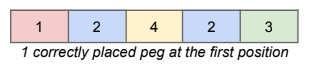
\includegraphics[width=0.5\linewidth]{question12.png}
\end{figure}
Feedback 1-1-C is given. Its corresponding event is (1-1-C). The entropy of $\mbox{S}_1$ has changed, because the probability distribution of the color of the first slot has changed. In fact, the probability of one of the color is equal to 1 and equal to 0 for all the other colors. Using the formula of the entropy and basic understanding of what the entropy is (no uncertainty $\Rightarrow$ no entropy), we know that
$$
\mbox{H}(\mbox{S}_1|(\mbox{1-1-C})) = 0 \mbox{ Shannon bit}
$$
As for the other slots, since we received no feedback about them, we know they can not be blue, yellow, or green. Therefore, slots 2, 3, 4, and 5 can only be red or brown, with equal probability, as there is no reason to favor one color over the other. Also, the entropy of slots 2, 3, 4, and 5 are equal, because their situations are identical. We compute their entropy using the formula  $\forall i \in \{2,3,4,5\}$
\begin{align*}
\mbox{H}(\mbox{S}_i|(\mbox{1-1-C})) &=- \sum_{j=1}^5\mbox{P}(\mbox{S}_i=j|(\mbox{1-1-C}))\log_2\mbox{P}(\mbox{S}_i=j|(\mbox{1-1-C})) \\
&= -(\mbox{P}(\mbox{S}_i=1|(\mbox{1-1-C}))\log_2\mbox{P}(\mbox{S}_i=1|(\mbox{1-1-C})) +\mbox{P}(\mbox{S}_i=5|(\mbox{1-1-C}))\log_2\mbox{P}(\mbox{S}_i=5|(\mbox{1-1-C}))) \\
&=-2\frac{1}{2}\log_2\left(\frac{1}{2}\right)\\
&=\log_2(2) \\
&= 1 \mbox{ Shannon bit}
\end{align*}

To compute $\mbox{H}(\mbox{M}|(\mbox{1-1-C}))$, we need to compute $\#(\mbox{M}=i, (\mbox{1-1-C}))$ and $\#((\mbox{1-1-C}))$. Firstly, there are five slots, and to be compatible with 1-1-C, the first slot of the configuration must be equal to 1, while the four other slots can take two equiprobable values independently of each other, so
$$
\#((\mbox{1-1-C}))=1\cdot2^4
$$
Let us define $\mbox{M}_{\mbox{1-1-C}}$ the set of all values of M that are compatible with 1-1-C. By definition, the cardinality of $\mbox{M}_{\mbox{1-1-C}} = \#((\mbox{1-1-C}))$. By definition of M, we deduce that
$$
\#(\mbox{M}=i, (\mbox{1-1-C}))=
\begin{cases}
       1 &\quad\text{if } i \in \mbox{M}_{\mbox{1-1-C}} \\
       0 &\quad\text{if } i \not\in \mbox{M}_{\mbox{1-1-C}}
     \end{cases}
$$
Let us compute the entropy of $\mbox{M}|(\mbox{1-1-C})$

\begin{align*}
    \mbox{H}(\mbox{M}|(\mbox{1-1-C})) =& \begin{multlined}
        -\sum_{i=1}^{\#(/)} \mbox{P}(\mbox{M}=i|(\mbox{1-1-C}))\log_2\mbox{P}(\mbox{M}=i|(\mbox{1-1-C}))
    \end{multlined}\\
    =& \begin{multlined}[t]
        -\hspace{-0.5cm}\sum_{\hspace{0.4cm}i\tiny\in\mbox{M}_{\mbox{1-1-C}}}\hspace{-0.45cm}\mbox{P}(\mbox{M}=i|(\mbox{1-1-C}))\log_2\mbox{P}(\mbox{M}=i|(\mbox{1-1-C})) \\- \hspace{-0.5cm}\sum_{\hspace{0.4cm}i\tiny\not\in\mbox{M}_{\mbox{1-1-C}}}\hspace{-0.45cm}\mbox{P}(\mbox{M}=i|(\mbox{1-1-C}))\log_2\mbox{P}(\mbox{M}=i|(\mbox{1-1-C}))
    \end{multlined}\\
    =& \begin{multlined}[t]
        -\hspace{-0.5cm}\sum_{\hspace{0.4cm}i\tiny\in\mbox{M}_{\mbox{1-1-C}}}\hspace{-0.45cm}\frac{\#(\mbox{M}=i, (\mbox{1-1-C}))}{\#((\mbox{1-1-C}))}\log_2\frac{\#(\mbox{M}=i, (\mbox{1-1-C}))}{\#((\mbox{1-1-C}))} \\- \hspace{-0.5cm}\sum_{\hspace{0.4cm}i\tiny\not\in\mbox{M}_{\mbox{1-1-C}}}\hspace{-0.45cm}\frac{\#(\mbox{M}=i, (\mbox{1-1-C}))}{\#((\mbox{1-1-C}))}\log_2\frac{\#(\mbox{M}=i, (\mbox{1-1-C}))}{\#((\mbox{1-1-C}))}
    \end{multlined}\\
    =& \begin{multlined}
        -\hspace{-0.5cm}\sum_{\hspace{0.4cm}i\tiny\in\mbox{M}_{\mbox{1-1-C}}}\hspace{-0.45cm}\frac{1}{\#((\mbox{1-1-C}))}\log_2\frac{1}{\#((\mbox{1-1-C}))}
    \end{multlined}
\end{align*}

Now, we use the value of the $\#((\mbox{1-1-C}))$ and the cardinality of $\mbox{M}_{\mbox{1-1-C}}$
\begin{align*}
    \mbox{H}(\mbox{M}|(\mbox{1-1-C})) &=-\hspace{-0.5cm}\sum_{\hspace{0.4cm}i\tiny\in\mbox{M}_{\mbox{1-1-C}}}\hspace{-0.45cm}\frac{1}{\#((\mbox{1-1-C}))}\log_2\frac{1}{\#((\mbox{1-1-C}))}\\
    &= -\#((\mbox{1-1-C})) \frac{1}{\#((\mbox{1-1-C}))}\log_2\frac{1}{\#((\mbox{1-1-C}))}\\
    &= \log_2\#((\mbox{1-1-C}))\\
    &=\log_2\left(2^4\right)\\
    &=4\log_2(2)\\
    &=4\mbox{ Shannon bits}
\end{align*}
Again, we have the following equality
\begin{align*}
\mbox{H}(\mbox{M}|(\mbox{1-1-C})) &= \mbox{H}(\mbox{S}_1, \mbox{S}_2, \mbox{S}_3, \mbox{S}_4, \mbox{S}_5|(\mbox{1-1-C}))\\
&= \mbox{H}(\mbox{S}_1|(\mbox{1-1-C})) + \mbox{H}(\mbox{S}_2|(\mbox{1-1-C})) + \mbox{H}(\mbox{S}_3|(\mbox{1-1-C})) + \mbox{H}(\mbox{S}_4|(\mbox{1-1-C})) + \mbox{H}(\mbox{S}_5|(\mbox{1-1-C}))
\end{align*}
so we can conclude that the $\mbox{S}_i$ remain independent after the guess.
\\\\
To compute the quantity of information that the guess brought, we just compute the difference between the entropy of the game before and after the feedback
$$
\mbox{H}(\mbox{M}) - \mbox{H}(\mbox{M}|(\mbox{1-1-C))} = 5\log_2(5) -4= 7.61\mbox{ Shannon bits}
$$
\subsection*{Question 13}
\begin{figure}[H]
    \centering
    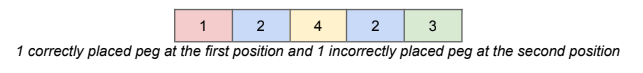
\includegraphics[width=1\linewidth]{question13.png}
\end{figure}
Feedback 1-1-C and 2-2-I are occurring. The event corresponding to the conjunction of feedback 1-1-C and feedback 2-2-I is $(\mbox{1-1-C}, \mbox{2-2-I})$. The probability distribution of $\mbox{S}_1$ does not change from the question 12, so its entropy does
$$
\mbox{H}(\mbox{S}_1|(\mbox{1-1-C},\mbox{2-2-I})) = \mbox{H}(\mbox{S}_1|(\mbox{1-1-C})) = 0 \mbox{ Shannon bit}
$$
First, notice that we received no feedback for slots three and five, so there is no yellow or green in the code. Also, there can only be one blue in the code; Otherwise, slot four would also be incorrect (4-2-I).
\\\\
The probability distribution of $\mbox{S}_2$ and  $\mbox{S}_4$ change. Indeed, they can only be red or brown, with equal probability, as there is no reason to favor one color over the other. Also, the entropy of slots two and four are equal, because their situations are identical. We compute their entropy using the formula  $\forall i \in \{2,4\}$
\begin{align*}
    \mbox{H}(\mbox{S}_i|(\mbox{1-1-C},\mbox{2-2-I}))=&\begin{multlined}[t]
        - \sum_{j=1}^5\mbox{P}(\mbox{S}_i=j|(\mbox{1-1-C},\mbox{2-2-I}))\log_2\mbox{P}(\mbox{S}_i=j|(\mbox{1-1-C},\mbox{2-2-I}))
    \end{multlined}\\
    =&\begin{multlined}[t]
    -(\mbox{P}(\mbox{S}_i=1|(\mbox{1-1-C},\mbox{2-2-I}))\log_2\mbox{P}(\mbox{S}_i=1|(\mbox{1-1-C},\mbox{2-2-I})) +\\ \mbox{P}(\mbox{S}_i=5|(\mbox{1-1-C},\mbox{2-2-I}))\log_2\mbox{P}(\mbox{S}_i=5|(\mbox{1-1-C},\mbox{2-2-I}))  )
    \end{multlined}\\
    =&\begin{multlined}[t]
    -2\frac{1}{2}\log_2\left(\frac{1}{2}\right)
    \end{multlined}\\
    =&\begin{multlined}
        \log_2(2)
    \end{multlined}\\
    =&\begin{multlined}
        1 \mbox{ Shannon bit}
    \end{multlined}\\
\end{align*}

Now, we compute $\mbox{H}(\mbox{S}_3|(\mbox{1-1-C},\mbox{2-2-I}))$ and $\mbox{H}(\mbox{S}_5|(\mbox{1-1-C},\mbox{2-2-I}))$ . Since the situations of $\mbox{S}_3$ and $\mbox{S}_5$ are symmetrical (We have the exact same informations about slots three and five), we know that
$$
\mbox{H}(\mbox{S}_3|(\mbox{1-1-C},\mbox{2-2-I})) = \mbox{H}(\mbox{S}_5|(\mbox{1-1-C},\mbox{2-2-I}))
$$
To compute $\mbox{H}(\mbox{S}_3|(\mbox{1-1-C},\mbox{2-2-I}))$, we need to compute 
$$
\mbox{P}(\mbox{S}_3=i|(\mbox{1-1-C},\mbox{2-2-I}))\; \forall i\in\{1,2,3,4,5\}
$$
We know that they can not be yellow or green, so
\begin{align*}
\mbox{P}(\mbox{S}_3=3|(\mbox{1-1-C},\mbox{2-2-I})) &= \mbox{P}(\mbox{S}_3=4|(\mbox{1-1-C},\mbox{2-2-I}))=0
\end{align*}
Again, we can not distinguish color brown and red in this case, so
\begin{align*}
\mbox{P}(\mbox{S}_3=1|(\mbox{1-1-C},\mbox{2-2-I})) &= \mbox{P}(\mbox{S}_3=5|(\mbox{1-1-C},\mbox{2-2-I})) =\frac{1}{2} \mbox{P}(\mbox{S}_3\not=2|(\mbox{1-1-C},\mbox{2-2-I}))
\end{align*}

Let us compute $\mbox{P}(\mbox{S}_3=2|(\mbox{1-1-C},\mbox{2-2-I}))$
$$
\mbox{P}(\mbox{S}_3=2|(\mbox{1-1-C},\mbox{2-2-I})) = \frac{\#(\mbox{S}_3=2,(\mbox{1-1-C},\mbox{2-2-I}))}{\#((\mbox{1-1-C},\mbox{2-2-I}))}
$$
Let us compute $\#((\mbox{1-1-C},\mbox{2-2-I}))$. 1-1-C and 2-2-I imply that $\mbox{S}_1$ is red, that $\mbox{S}_2$ and $\mbox{S}_4$ are either red, or brown, and that $(\mbox{S}_3 =2)\oplus(\mbox{S}_5=2)$. There is only one possibility for the value of $\mbox{S}_1$, two equiprobable values for $\mbox{S}_2$ and $\mbox{S}_4$ and the number of pairs ($\mbox{S}_3, \mbox{S}_5$) that contain exactly one color blue is equal to 4, because one slot will be blue and the other will be either red or brown (blue-red, blue-brown, red-blue, brown-blue). We conclude that
$$
\#((\mbox{1-1-C},\mbox{2-2-I}) )= 1\cdot2\cdot2\cdot4 
$$
We compute $\#(\mbox{S}_3=2,\mbox{1-1-C},\mbox{2-2-I})$ in the same way. The only difference is that the number of pairs ($\mbox{S}_3,\mbox{S}_5$) that contain exactly one blue slot is equal to 2, because $\mbox{S}_3$ takes the value 2 and $\mbox{S}_5$ will be either red or brown (blue-red, blue-brown).
$$
\#(\mbox{S}_3=2,(\mbox{1-1-C},\mbox{2-2-I}))=1\cdot2\cdot2\cdot2
$$
and so
$$
\mbox{P}(\mbox{S}_3=2|(\mbox{1-1-C},\mbox{2-2-I})) = \frac{\#(\mbox{S}_3=2,(\mbox{1-1-C},\mbox{2-2-I}))}{\#(\mbox{(1-1-C},\mbox{2-2-I}))} = \frac{1\cdot2\cdot2\cdot2}{1\cdot2\cdot2\cdot4 }=\frac{1}{2}
$$
Because
$$
\mbox{P}(\mbox{S}_3\not=2|(\mbox{1-1-C},\mbox{2-2-I})) + \mbox{P}(\mbox{S}_3=2|(\mbox{1-1-C},\mbox{2-2-I})) = 1
$$
we know that
$$
\mbox{P}(\mbox{S}_3\not=2|(\mbox{1-1-C},\mbox{2-2-I})) = 1-\mbox{P}(\mbox{S}_3=2|(\mbox{1-1-C},\mbox{2-2-I})) = 1 - \frac{1}{2} = \frac{1}{2}
$$
and that 
\begin{align*}
\mbox{P}(\mbox{S}_3=1|(\mbox{1-1-C},\mbox{2-2-I})) &= \mbox{P}(\mbox{S}_3=5|(\mbox{1-1-C},\mbox{2-2-I})) =\frac{1}{2} \mbox{P}(\mbox{S}_3\not=2|(\mbox{1-1-C},\mbox{2-2-I})) = \frac{1}{4}
\end{align*}
Now, we just use the entropy formula
\begin{align*}
\mbox{H}(\mbox{S}_3(|\mbox{1-1-C},\mbox{2-2-I})) &= -\sum_{i\in\{1,2,3,4,5\}}\mbox{P}(\mbox{S}_3=i|(\mbox{1-1-C},\mbox{2-2-I}))\log_2\mbox{P}(\mbox{S}_3=i|(\mbox{1-1-C},\mbox{2-2-I}))\\
&=-\sum_{i\in\{1,2,5\}}\mbox{P}(\mbox{S}_3=i|(\mbox{1-1-C},\mbox{2-2-I}))\log_2\mbox{P}(\mbox{S}_3=i|(\mbox{1-1-C},\mbox{2-2-I}))\\
&= -\left(\frac{1}{4}\log_2\left(\frac{1}{4}\right) + \frac{1}{2}\log_2\left(\frac{1}{2}\right) + \frac{1}{4}\log_2\left(\frac{1}{4}\right) \right)\\
&=-\frac{1}{2}\left(\log_2\left(\frac{1}{4}\right) + \log_2\left(\frac{1}{2}\right)\right)\\
&=\frac{1}{2} (\log_2(4) + \log_2(2))\\
&=\frac{1}{2}(2+1)\\
&=1.5 \mbox{ Shannon bit}
\end{align*}
To compute $\mbox{H}(\mbox{M}|(\mbox{1-1-C}, \mbox{2-2-I}))$, we need the values of $\#(\mbox{M}=i, (\mbox{1-1-C}, \mbox{2-2-I}))$ and $\#((\mbox{1-1-C}, \mbox{2-2-I}))$. We already know 
$$
\#((\mbox{1-1-C}, \mbox{2-2-I})) = 1\cdot2\cdot2\cdot4  = 16
$$
Let us define $\mbox{M}_{\mbox{1-1-C},\mbox{2-2-I}}$ the set of all values of M that are compatible with 1-1-C and 2-2-I. By definition, the cardinality of $\mbox{M}_{\mbox{1-1-C},\mbox{2-2-I}} = \#((\mbox{1-1-C}, \mbox{2-2-I}))$. By definition of M, we deduce that
$$
\#(\mbox{M}=i, (\mbox{1-1-C},\mbox{2-2-I}))=
\begin{cases}
       1 &\quad\text{if } i \in \mbox{M}_{\mbox{1-1-C},\mbox{2-2-I}} \\
       0 &\quad\text{if } i \not\in \mbox{M}_{\mbox{1-1-C},\mbox{2-2-I}}
     \end{cases}
$$
Let us compute the entropy of $\mbox{M}|(\mbox{1-1-C},\mbox{2-2-I})$. We proceed in the exact same way as in question 12.
\begin{align*}
    \mbox{H}(\mbox{M}|(\mbox{1-1-C},\mbox{2-2-I})) &= -\sum_{i=1}^{\#(/)} \mbox{P}(\mbox{M}=i|(\mbox{1-1-C},\mbox{2-2-I}))\log_2\mbox{P}(\mbox{M}=i|(\mbox{1-1-C},\mbox{2-2-I}))\\
    &\dots\\
    &=\log_2\#((\mbox{1-1-C},\mbox{2-2-I}))\\
    &=\log_2(16)\\
    &=4 \mbox{ Shannon bits}
\end{align*}
Let us compute the sum of the entropy of the slots
\begin{align*}
\begin{multlined}
    \mbox{H}(\mbox{S}_1|(\mbox{1-1-C},\mbox{2-2-I))} + \mbox{H}(\mbox{S}_2|(\mbox{1-1-C},\mbox{2-2-I))}+\mbox{H}(\mbox{S}_3|(\mbox{1-1-C},\mbox{2-2-I))}\\+\mbox{H}(\mbox{S}_4|(\mbox{1-1-C},\mbox{2-2-I))}+\mbox{H}(\mbox{S}_5|(\mbox{1-1-C},\mbox{2-2-I))} = 0 + 1 + 1.5 + 1 + 1.5 = 5 \mbox{ Shannon bits}
\end{multlined}
\end{align*}
As we can see, the sum of the entropy of the five slots is not equal to the entropy of the entire game, so we can deduce that the five slots are not independent anymore, due to the conjunction of 1-1-C and 2-2-I. Also, we can see that the entropy of the game is smaller than the sum of the entropy of the five slots. This is expected, because for any n random variables $\mathcal{X}_1,\dots,\mathcal{X}_n$
$$
\mbox{H}(\mathcal{X}_1,\dots,\mathcal{X}_n) \leq \sum_{i=1}^n \mbox{H}(\mathcal{X}_i)
$$
with the equality holding when the n variables are independent. Let us compute the quantity of information that the guess brought
$$
\mbox{H}(\mbox{M}) - \mbox{H}(\mbox{M}|(\mbox{1-1-C},\mbox{2-2-I})) = 5\log_2(5) - 4 = 7.61 \mbox{ Shannon bits}
$$
As we can see, the information gain in question 13 is equal to the one in question 12. It might seem unexpected that we gained the same quantity of information in both cases because the feedback from question 13 appears to provide more information (the feedback contains two statements, instead of one), and we might even be tempted to write
$$
\mbox{H}(\mbox{M}|\mbox{1-1-C},\mbox{2-2-I}) \leq \mbox{H}(\mbox{M}|\mbox{1-1-C})
$$
with the equality holding when $\mbox{M} \,\bot \,\mbox{2-2-I} |\mbox{1-1-C}$. However, it make no sense, because 1-1-C and 2-2-I are feedback and not events. In consequence, the set of configurations compatible with 1-1-C and 2-2-I is not a subset of the set of configurations compatible with 1-1-C (e.g. red-red-blue-red-red is compatible with 1-1-C and 2-2-I, but not with only 1-1-C), while it should be the case if 1-1-C and 2-2-I were truly events. Because the gain in entropy is equal in both questions, we can conclude that we have as much uncertainty about the code with both feedback.
\subsection*{Question 14}
Obviously, the maximum entropy can only be reach when we have not made any guess, because guesses can only reduce entropy by providing information.
\\\\
In this case, we have $\mathcal{S}$ slots that can take $\mathcal{C}$ values independently of each other, so $\#(/) = \mathcal{C}^\mathcal{S}$. Now, we define
$$
p_i=\mbox{P}(\mbox{M}=i)
$$
\begin{align*}
    \mbox{H}(\mbox{M}) &= -\sum_{i=1}^{\#(/)} \mbox{P}(\mbox{M}=i)\log_2\mbox{P}(\mbox{M}=i)\\
    &=-\sum_{i=1}^{\#(/)} p_i\log_2p_i\\
    &=\mbox{H}_{\#(/)}\left(p_1,\dots,p_{\#(/)}\right)\\
\end{align*}
We know a theorem about the entropy function
$$
\mbox{H}_n(p_1,\dots,p_n) \leq \log_2(n), \mbox{ with equality}\; \Leftrightarrow \forall i:p_i = \frac{1}{n}
$$
We apply it in our case to prove that
$$
    \mbox{H}(\mbox{M}) =\mbox{H}_{\#(/)}\left(p_1,\dots,p_{\#(/)}\right) \leq \log_2\#(/) = \log_2\mathcal{C}^\mathcal{S} = \mathcal{S}\log_2\mathcal{C}
$$
So if all Mastermind configurations are equiprobable, as we supposed in the previous questions, the entropy is maximal and is equal to $\mathcal{S}\log_2\mathcal{C}$.
\\\\
As expected, both the number of colors and the number of slots make the entropy of the game increases. Something interesting to point out is the fact that an increase of the number of slots has a greater impact on the maximum entropy than an increase of the number of colors: the maximum entropy increases linearly with the number of slots and logarithmically with the number of colors.
\subsection*{Question 15}
We would like to solve the general setting, so we must take into account the previous feedback. To do so, we totally ignore code which are not compatible with previous feedback. We denote $\mbox{M}_{\mbox{PF}}$, the set of all configurations which are compatible with the previous feedback. $\left|\mbox{M}_{\mbox{PF}} \right|$ denotes the cardinality of $\mbox{M}_{\mbox{PF}}$.
\\\\
Given a code and a guess, each slot can be assigned to one of three values: Correct (C), Incorrect (I), or Nothing (N). When the opponent communicates a feedback, he communicates a $\mathcal{S}\mbox{-tuple}$ $\left\{\mbox{C},\mbox{I},\mbox{N}\right\}^\mathcal{S}$. However, given a guess, multiple of these $\mathcal{S}\mbox{-tuple}$ can be equivalent. For example, at question 13, $(\mbox{C},\mbox{I},\mbox{N},\mbox{N},\mbox{N})$ and $(\mbox{C},\mbox{N},\mbox{N},\mbox{I},\mbox{N})$ are equivalent.
We define $\mbox{F}(\mbox{m},g)$, the set of equivalent $\mathcal{S}\mbox{-tuples}$ that can be given to a guess g, when the code is m. We define $\mbox{F}(\mbox{g}) = \{\mbox{F}(\mbox{m},\mbox{g})|\mbox{m} \in \mbox{M}_{\mbox{PF}}\}$.  An information-based approach would be to make the guess that minimizes the uncertainty about the code given the feedback. 
$$
\mbox{arg}\min_{\mbox{g}}\mbox{H}(\mbox{M}|\mbox{F}(\mbox{M},\mbox{g}))
$$
$\mbox{F}(\mbox{M},\mbox{g})$ is a random variable, since it is a function of the random variable M. For two random variables $\mathcal{X}$ and $\mathcal{Y}$, we know that (equivalent of bayes formula for entropy)
$$
\mbox{H}(\mathcal{X}|\mathcal{Y}) = \mbox{H}(\mathcal{Y}|\mathcal{X}) + \mbox{H}(\mathcal{X}) -\mbox{H}(\mathcal{Y})
$$
We apply this formula to our case
$$
\mbox{arg}\min_{\mbox{g}}\mbox{H}(\mbox{M}|\mbox{F}(\mbox{M},\mbox{g})) = \mbox{arg}\min_{\mbox{g}}\left(\mbox{H}(\mbox{F}(\mbox{M},\mbox{g})|\mbox{M}) + \mbox{H}(\mbox{M}) - \mbox{H}(\mbox{F}(\mbox{M},\mbox{g}) \right)
$$

If we know M, then $\mbox{F}(\mbox{M},\mbox{g})$ is known, so
$\mbox{H}(\mbox{F}(\mbox{M},\mbox{g})|\mbox{M}) = 0$, and because $\mbox{H}(\mbox{M})$ does not depend on g, we can ignore it.
$$
\mbox{arg}\min_{\mbox{g}}\mbox{H}(\mbox{M}|\mbox{F}(\mbox{M},\mbox{g})) = \mbox{arg}\min_{\mbox{g}}-\mbox{H}(\mbox{F}(\mbox{M},\mbox{g})) = \mbox{arg}\max_{\mbox{g}}\mbox{H}(\mbox{F}(\mbox{M},\mbox{g}))
$$
We obtain a simple rule: if we want to maximize our information gain on the code, we must choose a guess that maximize the expected quantity of information in the feedback. Using the formula of the entropy
\begin{align*}
    \mbox{H}(\mbox{F}(\mbox{M},\mbox{g})) &= -\sum_{f\in\mbox{F}(\mbox{g})} \mbox{P}(\mbox{F}(\mbox{M},\mbox{g}) = f) \log_2\mbox{P}(\mbox{F}(\mbox{M},\mbox{g}) = f)
\end{align*}
And we can compute 
$$\mbox{P}(\mbox{F}(\mbox{M},\mbox{g}) = f) = \frac{\#(\mbox{F}(\mbox{M},\mbox{g}) = f)}{\left|\mbox{M}_{\mbox{PF}}\right|}
$$
We can compute $\mbox{H}(\mbox{F}(\mbox{M},\mbox{g}))$ for all possible guess and pick the one that lead to the greatest value. $\mbox{F}(\mbox{m},\mbox{g})$ can be easily (not efficiently) computed for each m by verifying which feedback is compatible with m and g. Then, $\mbox{F}(\mbox{g})$ can be easily obtained from the $\mbox{F}(\mbox{m},\mbox{g})$. Finally, $\#(\mbox{F}(\mbox{M},\mbox{g}) = f)$ can be computed by iterating on the set of configurations $\mbox{M}_{\mbox{PF}}$ and using the $\mbox{F}(\mbox{m},\mbox{g})$ previously computed. This naive approach is inefficient, but it is sound and complete.
\end{document}
